\chapter{Fazit und Ausblick}
Das Ziel dieser Arbeit war ein verteiltes 3D-Echtzeit-Renderingsystem zu entwicklen, dass in der Lage ist eine 3D-Szene mit Hilfe von WebGL auf dem Client darzustellen und an ein Realtime Interactive System angebunden ist. Hierzu wurden ein WebGL-Renderer, eine serverseitige Webanwendung auf Basis des Play! Frameworks und die Anbindung an ein bestehendes RIS vollständig neu implementiert.
\begin{figure}
\centering
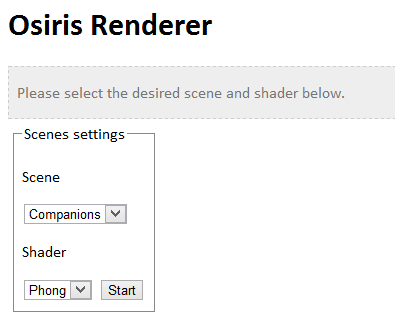
\includegraphics[width=90mm]{bilder/osirissettings.png}
\caption{Auswahl der zu rendernden Szene und des Shaderprogramms}
\label{fig:osirissettings}
\end{figure}

Die wesentliche Herausforderung war die Interaktion der unterschiedlichen Technologien untereinander sicher zu stellen, was eine intensive Einarbeitung in die einzelnen Wissensfelder erforderte.

Insbesondere die Anbindung an SIRIS, das verwendete RIS, gestaltete sich zuerst als schwierig da es bisher kaum dokumentiert ist. Im Endeffekt gestaltete sie sich nach der notwendigen Einarbeitungszeit in das System jedoch als überraschend einfach. Die Hauptaufgabe wird von einem SIRIS-Actor übernommen, der lediglich 148 Zeilen Quelltext lang ist. In kleinem Maßstab diente Osiris damit auch als Feldtest für die Entwicklung einer völlig neuartigen Komponente für das RIS.

Der WebGL-Renderer ist in der Lage vom Anwender gewählte Szenen mit unterschiedlichen Shaderprogrammen und dessen Interaktion mit den Objekten der Szene darzustellen und mit dem serverseitigen RIS zu kommunizieren. Allerdings muss auch festgesetllt werden, dass eine beliebige Kombination von Szenen und Shaderprogrammen nicht möglich ist. Der Renderer kann besipielsweise Szenen, die mehrere Lichtquellen eines Typs (mehrere Spotlichter beispielsweise) nicht darstellen. Da Shader völlig frei programmierbar sind, müsste hier deutlich mehr Aufwand betrieben werden, was jedoch im Rahmen dieser Arbeit weder Aufgabe noch zeitlich möglich gewesen wäre.

In der Planungsphase des Projekts gab es Bedenken, dass die Kommunikation zwischen dem clientseitigen Renderer und dem serverseitigen RIS nicht performant genug wäre, um eine Echtzeitinteraktion des Anwenders mit den Objekten der Szene und der Objekte untereinander zu realisieren. Letztendlich hat es sich jedoch herausgestellt, dass die Kommunikation mit (kleinen) JSON-Nachrichten über ein WebSocket zumindest für die derzeit in Osiris enthaltenen Szenen völlig ausreicht. Für eine realistische Einschätzung der Belastbarkeit und Leistungsfähigkeit wäre ein zukünftiger Performancetest mit sehr komplexen Szenen und vielen Objekten notwendig, welcher jedoch den zeitlichen Rahmen dieser Arbeit gesprengt hätte.
\begin{figure}
\centering
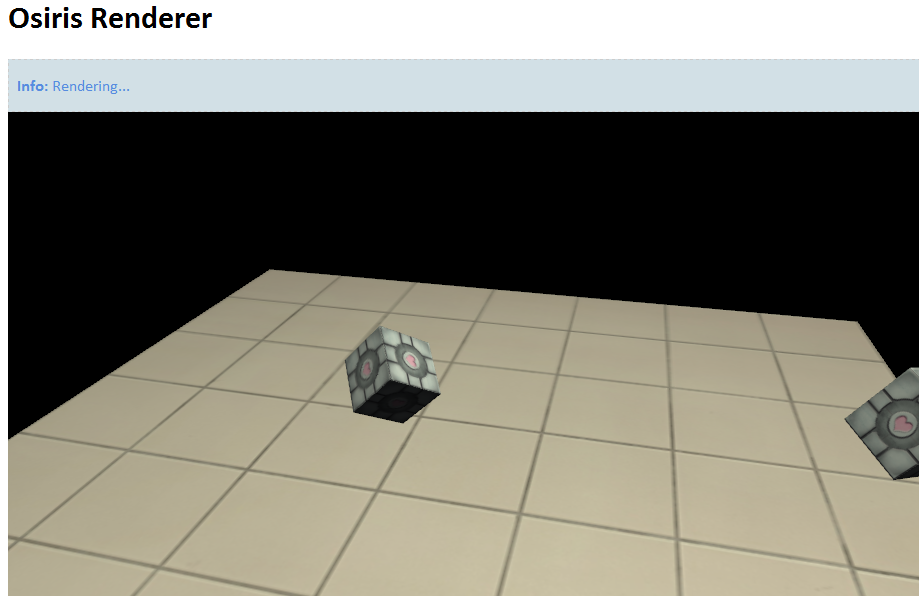
\includegraphics[width=\textwidth]{bilder/osiris.png}
\caption{Ein Bild des laufenden Renderers}
\label{fig:osiris}
\end{figure}

Die Wahl des Play! Frameworks als Grundlage für die serverseitige Webanwendung hat sich als sehr günstig erwiesen. Es bietet alle benötigten Strukturen an, ohne jedoch die Programmierung durch Konfigurationsaufwand oder umständliche Verwendung zu behindern. Tatsächlich waren die Controller für die statischen Ressourcen und die WebSocket-Verbindung sehr zeitnah implementiert. Aufgrund seiner Architektur und des statuslosen Zustands bei Anfragen ist es einerseits möglich Anwendungen ohne größeren Aufwand schnell zu skalieren und es, wenn gewünscht, auch relativ leicht durch eine andere Lösung zu ersetzen. Leider hat der statuslose Zustand aber auch einen Nachteil, nämlich den höheren Zeitaufwand der nötig gewesen wäre, um eine Mehrbenutzerumgebung zu implementieren. Osiris ist in seinem aktuellen Prototypenstatus lediglich von einem Benutzer verwendbar.

In der Nachschau hätten einige Aspekte mit mehr Zeit besser gelöst werden können. Von der Schlichtheit der Gui mal abgesehen wäre beispielsweise zur Flexibilisierung des Shaderprogramms ein System besser, welches nicht direkt von den Attributes und Uniforms abhängt, sondern einer abstrakten Beschreibung der erwarteten Darstellung. Diese würde gelesen und zur Laufzeit daraus dynamisch ein passendes Shaderprogramm generiert werden. Auch wäre zur Leistungssteigerung eine vollständigere Umwandlung der vom Server geladenen Szene in einen nur noch die relevanten Teile enthaltenden und auf Traversierungsgeschwindigkeit optimierten Szenegraphen und das Aufteilen der Renderschleife in verschiedene Renderpasses günstig gewesen. Zur nochmaligen Verkleinerung der zwischen Client und Server ständig übertragenen Datenmenge könnte zudem das MessagePack-Format\footnote{\url{http://msgpack.org/} (besucht am \today)} statt JSON verwendet werden. Jedoch wären diese Verbesserungen in der kurzen Zeitspanne der Bachelorarbeit allein kaum möglich gewesen. Sie eröffnen jedoch Möglichkeiten auf dem gewonnenen Wissen aufzubauen.

Zusammenfassend kann die gestellte Aufgabe als vollständig gelöst betrachtet werden. Im Endergebnis konnte gezeigt werden, dass es durch die Verwendung von WebGL und der Anbindung an ein serverseitiges RIS möglich ist, 3D-Anwendungen zu entwickeln, die keine besonderen Anforderungen benötigen. Ein aktueller Browser wie Google Chrome oder Mozilla Firefox reicht völlig aus. Hierdurch ist die zugrundeliegende Systemarchitektur des Clients völlig unwichtig und der Anwender kann die Applikation direkt durch das Aufrufen einer URL nutzen.

